\section{Entre archives et documentation : une problématique propre aux musées}

Les musées en France, institutions dédiées à la conservation et à la diffusion du patrimoine, sont intimement liés à la question des archives : eux-même producteurs d'archives, ils peuvent être également exceptionnellement appelés à en être les dépositaires lorsqu'elles sont indissociables d'une oeuvre. Malgré la prégnance des problématiques liées à la gestion des archives dans les musées dans le paysage français, la littérature scientifique et professionnelle sur ce sujet semble peu prolifique : l'article de référence que nous retiendrons pour ce développement est celui de Véronique Sassetti-Aguilera, \citetitle{sassetti-aguileraArchivesMuseesDiversites2020a}. L'autrice identifie trois problématiques principales dans les musées actuellement : 

\begin{myquote}
	{La première difficulté réside dans le statut même de l'établissement (public ou privé) qui caractérise le plus souvent la nature des fonds d'archives et des collections [...] La deuxième, nettement plus complexe, relève de l'identification des archives par le personnel des musées comme trésors nationaux, imprescriptibles et inaliénables [...] La troisième enfin, et non la moindre, demeure dans l'enrichissement continuel de la documentation scientifique des collections de musées, situation ne permettant jamais [...] de procédures d'archivage classiques par bordereaux de versement.}{sassetti-aguileraArchivesMuseesDiversites2020a}
\end{myquote}. Où finit la documentation, où commence l'archive ? Cette interrogation se complique singulièrement dans l'environnement numérique muséal, où la nature hybride des fonds brouille les distinctions traditionnelles.

\subsection{Définir l’archive numérique en contexte muséal : enjeux et ambiguïtés}

\paragraph*{Documentation et archives}
Cette situation se retrouve ainsi particulièrement au \mae~: dans cette institution publique -- dont les archives produites sont donc des archives publiques, inaliénables selon le Livre II du \textit{Code du Patrimoine}, des informations sont en effet produites et récoltées dans une visée seulement scientifique de documentation et de contextualisation des collections. Cette documentation, à différencier des archives, est ainsi définie par le Ministère de la Culture dans ses recommandations aux musées : 
\begin{myquote}
	{La documentation est constituée par un ensemble d'informations de nature diverse réunies volontairement sur un thème donné afin de constituer une base de connaissances. Lorsque la documentation comprend des sources archivistiques, les informations contenues dans ces documents doivent être communiqués dans le respect des règles de communication}{ministeredelacultureDocumenterArchiverMusee2020}
\end{myquote}.

Comme démontré par Véronique Sasseti-Aguilera dans l'article cité précédemment, ou encore directement auprès de professionnels des musées au cours d'une session de formation comme celle proposée par la fédération des écomusées et des musées de société (FEMS)\footcite{federationdesecomuseesetmuseesdesocietefemsArchivesMusees2025}, il convient donc, dans tout musée, de bien différencier :
\begin{itemize}
	\item les archives conservées par le musées, qu'elles soient publiques ou privées lorsqu'elles proviennent de dons ou d'acquisitions à des fins de documentation des collections : celles-ci dépendent du Livre II du \textit{Code du Patrimoine} consacré aux archives, 
	\item de la documentation et des collections du musées qui dépendent donc du Livre IV du \textit{Code du Patrimoine} consacré aux musées.
\end{itemize}

\paragraph*{Des archives perpétuellement intermédiaires}
Véronique Sasseti-Aguilera identifie donc une dernière particularité des archives en musée -- qui touche tout autant les archives papier que numérique : \enquote{Elles ont \textelp{}, et de manière tout à fait exceptionnelle, l’âge perpétuel d’\gls{archiveintermediaire}\footnote{Pour plus d'informations sur ce sujet, voir dans le glossaire la \gls{theorie3ages}}, puisqu’elles sont détentrices d’une valeur supplémentaire aux valeurs probante ou historique du fait de leur attachement à un objet patrimonial.} Ceci représente un nouveau défi pour les musées qui doivent donc garantir l'accessibilité et la pérennité de ces documents qui seront donc, \textit{a priori}, toujours consultés au musée.

\paragraph*{Situation au \mae}
Le \mae~ne défraie pas à cette situation : les dossiers d’œuvre, bureautique, rapports, photographies, courriels et autres documents ne relevant pas de la documentation ont légalement le statut d’archives publiques, librement communicables à tout citoyen. Pour les archives numériques, la question prioritaire qui se pose aujourd'hui au \mae~n'est cependant pas tant de différencier la documentation des archives -- bien que l’ambiguïté demeure, par exemple en ce qui concerne les photos de campagnes de récolement ou la documentation historique liée à des expositions ou campagnes de restauration. Comment garantir l'accessibilité et la pérennité de ces informations lorsqu'il n'y a pas d'archiviste pour veiller à cette tâche ? 

\begin{figure}
	\centering
	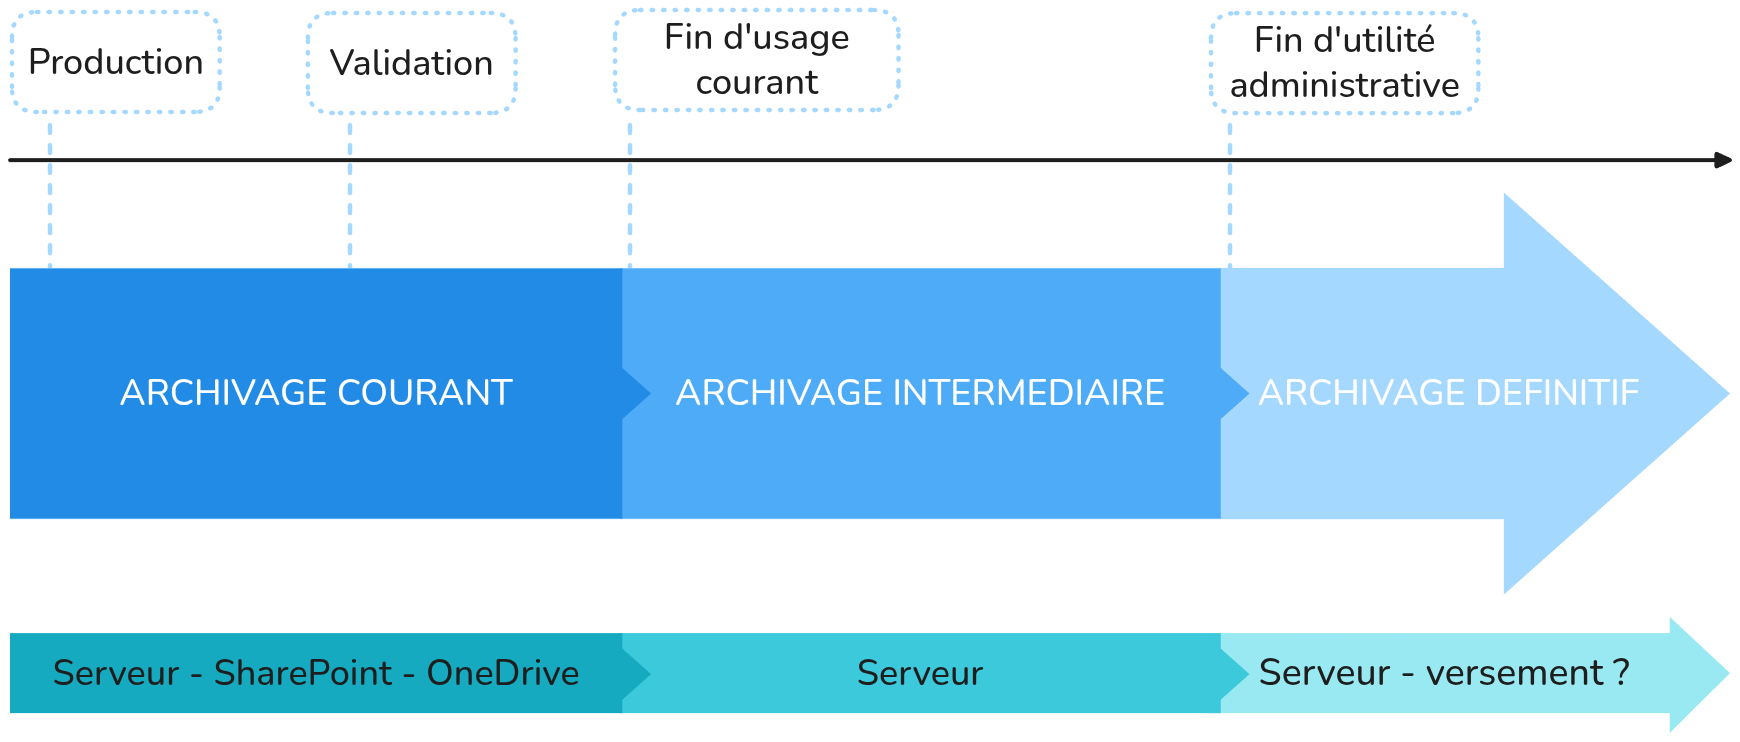
\includegraphics[width=0.7\linewidth]{img/SCHEM_theorie3ages}
	\caption[Cycle de vie des archives au \mae]{Schéma diffusé lors de la formation des 24 juin et 9 juillet 2025 : explication des la \gls{theorie3ages} et état actuel de la conservation des archives au musée.}
	\label{fig:schemtheorie3ages}
\end{figure}


\subsection{Panorama des pratiques de gestion des archives numériques au MAE}

Avant d’entrer dans le détail des pratiques de gestion des archives numériques au sein du musée, il convient de rappeler la méthode qui a permis d’établir ce panorama. Celui-ci s’appuie sur un double corpus : d’une part, les diagnostics techniques réalisés à l’aide de l’outil \gls{archifiltre} sur le dossier \textit{Conservation} du serveur principal, qui ont permis d’analyser l’état des espaces, la structure des dossiers et la répartition des fichiers ; d’autre part, les réponses recueillies auprès des agents du \ac{dsc} grâce à un questionnaire diffusé via Microsoft Forms. Ce croisement entre l'analyse automatisée et la perception des usagers tente d'offrir un éclairage nuancé sur les difficultés, les logiques d’organisation et les représentations qui président à la gestion des archives numériques au \mae. C’est à partir de cette matière que s’amorce l’état des lieux qui suit.

\paragraph*{Le stockage des fichiers au \mae}
Cette organisation se caractérise avant tout par la coexistence de multiples espaces de stockage\footnote{Aucune solution dédiée n'ayant été mise en place pour assurer la collecte, la conservation, le classement et la communication de ces archives, il a semblé plus exact de parler d'\enquote{espace de stockage} que d'\enquote{espace de conservation}} :

\begin{itemize}
	\item le serveur principal -- serveur "services", dit \enquote{Serveur S}--, pivot de la conservation courante, structure ses dossiers par service dans une arborescence gérée via l’explorateur \textit{Windows}. 
	\item des espaces partagés sur \textit{SharePoint} mis en place récemment et dont l'utilisation se répand peu à peu s'ajoutent à ce serveur pour les projets en cours ou la diffusion de documents à l'ensemble du musée à titre d'information,
	\item enfin, les postes individuels des agents sont enregistrés et synchronisés sur \textit{OneDrive}.
\end{itemize}

Pour partager les fichiers, deux solutions coexistent, qui peuvent amener à la création de doublons :

\begin{itemize}
	\item l'utilisation des outils de partage de \textit{Microsoft} (\textit{Teams}, mail, \textit{SharePoint}\dots),
	\item et la création ou le déplacement du fichier en question dans un dossier partagé sur le Serveur S.
	
\end{itemize}

Cette dispersion reflète la diversité des pratiques et des métiers : chaque agent et service façonne sa propre architecture documentaire, souvent sans concertation globale. De fait, l'une des premières difficultés liées aux archives numériques qui sont remontées lors des analyses d'arborescences et des consultations d'agents a été l'absence de méthodologie globale -- laissant les agents sans guide clair pour gérer leurs propres documents -- et sa conséquence directe, qui est la difficulté d'y retrouver certaines informations.

\begin{figure}
	\centering
	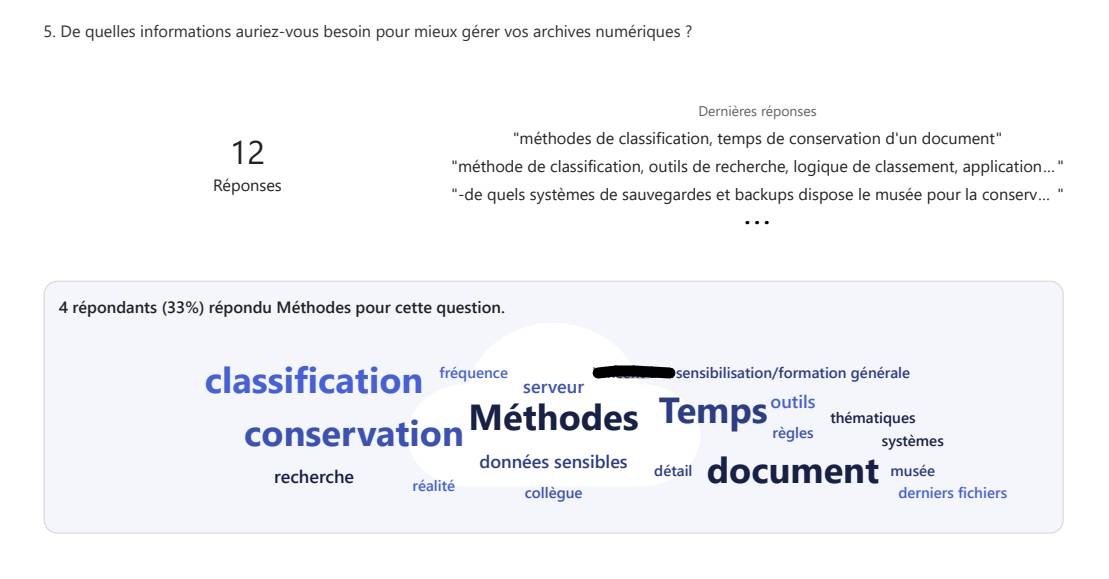
\includegraphics[width=0.7\linewidth]{img/IMG_questionnaire_attentes}
	\caption[Attentes des agents du \mae~en matière de gestion des archives]{Réponses des agents du musée à la question ... (nuage de mots généré par \textit{Microsoft Forms})}
	\label{fig:imgquestionnaireattentes}
\end{figure}

\paragraph*{Analyses du serveur}\footnote{Les graphiques et visualisations issues des analyses \gls{archifiltre} sont disponibles en annexe \refinterne{Ax-H}}
Les analyses du serveur font en effet écho à ces impressions : certaines branches du dossier Conservation, par exemple, atteignent jusqu’à seize niveaux de profondeur, dépassant de loin les recommandations habituelles\footnote{Un résumé de ces recommandations est disponible sur la documentation d'\gls{archifiltre} à l'adresse suivante : \cite{WikiArchifiltre}}. Une telle granularité rend l’information difficile à retrouver, la navigation labyrinthique, et allonge les chemins d’accès qui deviennent inexploitables par certains logiciels une fois franchie la limite des 256 caractères. À l’inverse, il existe aussi des dossiers quasi-vides dont la création procède d’une volonté de précision excessive, et qui contribuent à l'invisibilisation de certains documents dans le serveur à cause d'un surplus d'information dans l'arborescence. Cette situation s'explique surtout par l'absence d'un plan de classement partagé -- en effet, il n'existe pas d'autre contrainte à la création de fichiers que le \enquote{squelette} de dossiers par départements établis par le support informatique en racine du dossier Conservation.

Les conventions de nommage, fluctuantes, laissent coexister abréviations disparates, noms d’agents, ou intitulés vagues – autant de choix qui compromettent la pérennité et la fiabilité de l’information. Les « dossiers vrac », souvent mis en place faute de solution alternative, incarnent cette difficulté à organiser durablement la masse documentaire favorisent encore la perte de repères et nuisent à la circulation de l’information.


Le ratio moyen de fichiers par dossier, particulièrement flagrant dans les collections techniques, révèle ainsi l’ampleur du problème : là où la recommandation invite à dépasser dix fichiers par sous-dossier pour éviter de perdre des informations avec une arborescence trop granulaire, on observe une moyenne de 5,2 fichiers par dossiers, ce qui est signe d’une dispersion excessive et d’une structuration trop atomisée. Les doublons, qui saturent l’espace de stockage, atteignent jusqu’à 22\% du poids total du dossier dans certains cas, principalement du fait de la répétition d'images et de vidéos, souvent copiées d'un dossier à l'autre au gré des besoins de documentation des oeuvres du musée.


À cette fragmentation s’ajoute l’absence de solutions pour l’élimination et la conservation des fichiers : sans logiciel dédié à la gestion des archives ni solution de versement régulier des \gls{archivedefinitive} ni autorité référente active pour valider l'élimination de documents, la gestion des archives numériques dépend donc de l’initiative ou de la mémoire des agents, et des missions ponctuelles proposées par le \ac{drd}. La conséquence directe de cet état de fait est donc l’invisibilisation progressive des contenus, la multiplication des pertes d’information et l'accumulation des données sur des serveurs qui ne sont pas conçus pour remplir une mission de conservation et de partage de documents au sens archivistique. 



Ainsi, la multiplicité des espaces et la diversité des usages sont un obstacle à l'efficacité de la gestion des archives -- et donc d'une partie de la mémoire de l'institution : l’absence d’un cadre partagé, la prolifération des conventions individuelles et l’atomisation des pratiques font de la gestion documentaire un défi quotidien, que le musée ne peut relever sans une réflexion d’ensemble et une harmonisation concertée de ses outils et de ses méthodes.


\subsection{Une surcharge de travail pour le personnel du musée : la difficile reconnaissance de la fonction archivistique}


Dans l’organigramme du \mae, la fonction archivistique demeure résiduelle : une seule archiviste, arrivée en 2024, se consacre aux archives privées papier, elle est rattachée au \ac{drd}. L’absence, jusqu'à cette année, de politique de formation et de sensibilisation des personnels non archivistes accroît la difficulté à établir le plan de classement, le tableau de gestion ou la chaîne archivistique qui optimiseraient la gestion des archives numériques du musée.

\paragraph*{Dilution des responsabilités, surcharge des agents}
Les conséquences sont immédiates : organisation des dossiers, gestion des dossiers d’œuvres ou de la documentation, tout repose sur des agents dont l’expertise archivistique est souvent autodidacte et dont les missions sont bien éloignées de ces problématiques. Les pratiques de classement et d’élimination, pourtant encadrées par le code du patrimoine et les recommandations du \ac{siaf}, sont ainsi difficilement imposables à l'ensemble des agents au quotidien. L’uniformisation des procédures évoquée par Véronique Sassetti-Aguilera\footcite{sassetti-aguileraArchivesMuseesDiversites2020a}, reste un idéal, confronté à la faiblesse des moyens humains. Des missions ponctuelles de gestion des archives -- lors de stages longs ou de contrats courts -- ont pourtant été menées -- principalement pour répondre à des questions particulières comme une saturation du serveur ; mais malgré la volonté marquée du \ac{drd} et même de l'ensemble du \ac{dsc} d'agir dans le sens d'une rationalisation de la gestion des archives selon les recommandations en usage, aucune solution n'est encore proposée au niveau de l'institution.

La question de fond est celle de la légitimité : pourquoi la fonction archivistique demeure-t-elle marginale dans les musées, alors même que l’explosion des données numériques appelle une gouvernance renforcée ? Peut-on, à partir de l’exemple du \mae, réfléchir à l’élaboration de procédures spécifiques pour les archives publiques de musée en France ? En effet, bien que des groupes de travail de professionnels se soient formés pour répondre à cette question\footnote{Par exemple, le groupe de travail \enquote{Archives en musées} \cite{clergeauReseauArchivesMusees2015a}}, le sujet ne semble pas encore avoir touché l'ensemble des institutions concernées.
